\chapter{Clase 3}

\section{Unicidad en sucesiones acotadas}

 Dado $\varepsilon > 0$, $\exists\, k_0 \in \mathbb{N}$,  
tal que $k \geq k_0 \Rightarrow \|x_k - a\| < \varepsilon$

\begin{figure}[H]
	\centering
	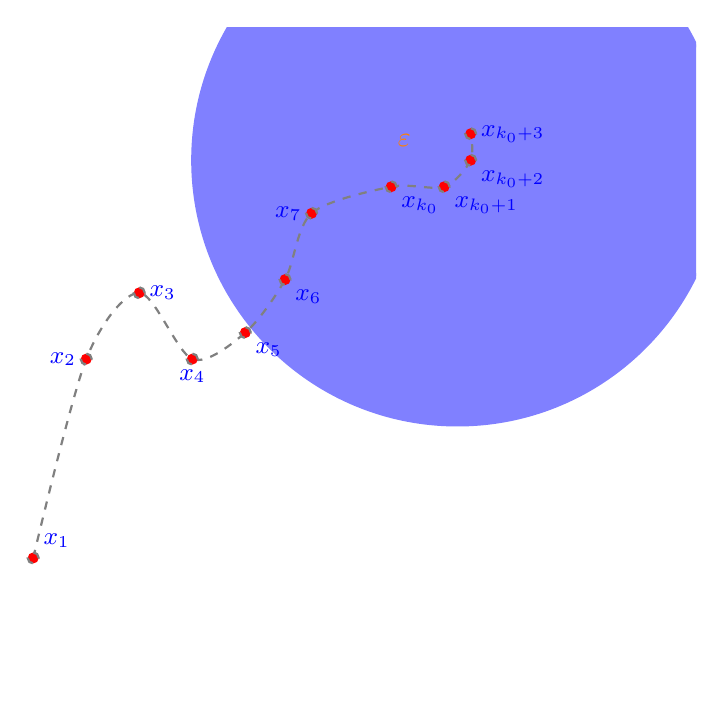
\begin{tikzpicture}[scale=1]
		\begin{axis}[
			width=10cm, height=10cm,
			%axis lines=middle,
			axis lines=none,
			xtick=\empty, ytick=\empty,
			axis equal,
			%enlargelimits,
			xmin=0, xmax=5,
			ymin=0, ymax=3,
			thick,
			xlabel={$x$}, ylabel={$y$},
			axis line style={->}
			]
			% circulo
			\draw[blue!50,fill=blue!50, thick] (axis cs:3.2,3) circle[radius=2];
			\draw[blue!50, ->] (axis cs:3.2,3) -- (axis cs:2.5,3.1); %radio
			
			% Punto límite a
			%\addplot[only marks, mark=*, mark options={fill=blue},  nodes near coords={$a$}, point meta=explicit symbolic ] coordinates { (3,3) [a] };
			
			% Bola abierta centrada en a
			\draw[orange, dashed, thick] (axis cs:3.2,3) circle[radius=70];
			\node[orange] at (axis cs:2.8,3.15) { $\varepsilon$};
			
			
			% Puntos de la sucesión fuera de la bola
			%\addplot[only marks, mark=*, mark options={fill=green} ] coordinates { 	(0,0) (0.5, 1.5) (0.9,2) (1.3, 1.5) (1.7,1.7)  (2.1,2.1)   (2.4, 2.6)   };
			
			% Puntos de la sucesión dentro de la bola
			%\addplot[only marks, mark=*,  mark options={fill=green} ] coordinates { 	(2.7,2.8)  (3.1,2.8)  (3.3,3) (3.3,3.2)  };
			\addplot+[smooth, dashed, gray, mark=*, mark options={fill=red}] coordinates {
				(0,0)        (0.4, 1.5) (0.8,2) (1.2, 1.5) (1.6,1.7) 
				(1.9,2.1)    (2.1, 2.6) (2.7,2.8) (3.1,2.8) (3.3,3) (3.3,3.2)
			};  
			
			% Etiquetas personalizadas
			\node[font=\small\bfseries, text=blue] at (axis cs:0,0)        [above right]  {$x_1$};
			\node[font=\small\bfseries, text=blue] at (axis cs:0.4,1.5)    [left]       {$x_2$};
			\node[font=\small\bfseries, text=blue] at (axis cs:0.8,2)      [  right] {$x_3$};
			\node[font=\small\bfseries, text=blue] at (axis cs:1.2,1.5)    [below]       {$x_4$};
			\node[font=\small\bfseries, text=blue] at (axis cs:1.6,1.7)    [ below right] {$x_5$};
			\node[font=\small\bfseries, text=blue] at (axis cs:1.9,2.1)    [below right]       {$x_6$};
			\node[font=\small\bfseries, text=blue] at (axis cs:2.1,2.6)    [  left]  {$x_7$};
			\node[font=\small\bfseries, text=blue]  at (axis cs:2.7,2.8)    [ below right]  {$x_{k_0}$};
			\node[font=\small\bfseries, text=blue]  at (axis cs:3.1,2.8)    [below right]       {$x_{k_0+1}$};
			\node[font=\small\bfseries, text=blue]  at (axis cs:3.3,3)      [below right]       {$x_{k_0+2}$};
			\node[font=\small\bfseries, text=blue]  at (axis cs:3.3,3.2)    [ right] {$x_{k_0+3}$};
			
			
		\end{axis}
	\end{tikzpicture} 
\end{figure}
\vspace{-6em} % o prueba -2em o -0.5em, según lo que necesites

\thmr{}{teorema3-1}{


Sea $(x_k)_{k\in \N} \subset \Rn$ una sucesión acotada. Entonces, $(x_k)_{k\in \N}$ es convergente si y sólo si toda subsucesión convergente de $(x_k)_{k\in \N}$ converge al mismo punto de $\Rn$.

}
\pf{Prueba del teorema \ref{thm:teorema3-1}
	
$(\Rightarrow)$  Supongamos que $\lim\limits_{k \to \infty} x_k = a \in \Rn$. Sea $(x_{i_k})_{k \in \N} \subset (x_k)_{k \in \N}$ una subsucesión.

\begin{equation}
 \forall \varepsilon > 0,\, \exists\, k_0 \in \N:\, \forall k \in \N,\; k \geq k_0 \Rightarrow \|x_k - a\| < \varepsilon    \label{eq:class3-1} 
\end{equation}

Como \((i_k)_{k \in \N} \subset \N\) es estrictamente creciente \(\Rightarrow i_k \geq k,\, \forall k \in \N\).

Entonces, \(k \geq k_0 \Rightarrow i_k \geq k \geq k_0 \Rightarrow \|x_{i_k} - a\| < \varepsilon\) por \eqref{eq:class3-1}.

\(\therefore \lim\limits_{k \to \infty} x_{i_k} = a\).  


($\Leftarrow$) Supongamos que toda subsucesión de $(x_k)_{k\in \N}$ que converge lo hace al mismo punto.

Sea $A = \qty{a \in \Rn, \exists \, (x_{i_k})_{k\in \N} \subset (x_k)_{k\in \N} : \lim\limits_{k \to \infty } x_{i_k}=a}$ (Conjunto de valores de adherencia de la sucesión $(x_k)_{k\in\N}$)

Como $(x_k)_{k\in \N}$ es acotada, del teorema de \textbf{Bolzano-Weierstrass}, $\exists (x_{i_k})_k \subset (x_k)_k$ tal que $\lim\limits_{k \to \infty } x_{i_k}=a \in \Rn$. Así $ a\in A, A \neq  \varnothing $

Queremos mostrar que $\lim\lim_{k \to \infty} x_k=a$

Por reducción al absurdo, supongamos que \underline{no ocurra} $\lim\limits_{k \to \infty} x_k=a$

$$
\sim( \forall \varepsilon > 0,\, \exists\, k_0 \in \N:\, \forall k \in \N,\; k \geq k_0 \Rightarrow \|x_k - a\| < \varepsilon )
$$
$$
 \exists\, \varepsilon > 0,\, \forall\, k_0 \in \N:\, \exists\, k \in \N,\; k \geq k_0 \wedge \|x_k - a\| \geq \varepsilon 
$$

Podemos construir $(x_{j_k})_{k\in\N} \subset (x_k)_{k\in \N}$ tal que
\begin{equation}
	 \abs{x_{i_j}-a}\geq \varepsilon_0 \quad\forall k\in \N \label{eq:class3-eq2}
\end{equation}  

Por el teorema de \textbf{Bolzano-Weierstrass}, \(\exists\, \pqty{x_{j_{p_k}}}_{k \in \N} \subset (x_{j_k})_{k \in \N}\) tal que 
\[
\lim\limits_{k \to \infty} x_{j_{p_k}} = b \in \Rn
\]
De \eqref{eq:class3-eq2} $\abs{ x_{j_{p_k}} -a} \geq \varepsilon_0, \quad \forall k \in \N$

Así, $\abs{b-a} = \lim\limits_{k \to \infty}\abs{ x_{j_{p_k}}-a} = \varepsilon_0 >0 \rightarrow b\neq a$
}

\section{Puntos de acumulación}

